\documentclass[polish]{article}



\usepackage{polski}
\usepackage[T1]{fontenc}
\usepackage{tgpagella}
\usepackage{colortbl}
\usepackage[table]{xcolor}
% \usepackage[a4paper, total={7in, 10in}]{geometry}
\usepackage[a4paper, left=0.75in, right=0.75in, top=0.75in, bottom=0.75in]{geometry}
\usepackage{listings}
\usepackage{titlesec}
\usepackage{graphicx}
\usepackage[autostyle]{csquotes}
\DeclareQuoteAlias{dutch}{polish}
\usepackage[utf8]{inputenc}
\usepackage{babel}
\usepackage{soul}
\usepackage{indentfirst}
\usepackage{fancyhdr}
\usepackage{xcolor}
\usepackage{lipsum}
\usepackage{enumitem}
\usepackage{float}
\usepackage{amsmath}
\usepackage{hyperref}
\usepackage[normalem]{ulem}

\hypersetup{
    colorlinks=true,
    citecolor=black,
    filecolor=black,
    linkcolor=black,
    urlcolor=black
}

\setlength\parindent{24pt}


\titlelabel{\thetitle.\quad}


\lstset
{
    %basicstyle=\footnotesize,
    backgroundcolor=\color{black!5}, % set backgroundcolor
    basicstyle=\footnotesize\small,% basic font setting
    %basicstyle=\sffamily,
    numbers=left,
    stepnumber=0,
    showstringspaces=false,
    tabsize=1,
    breaklines=true,
    breakatwhitespace=false,
}

\lstnewenvironment{CPP}
  {\lstset{
    language=C++,
    backgroundcolor=\color{black!5}, % set backgroundcolor
    basicstyle=\footnotesize\small,% basic font setting
    commentstyle=\color{green!60!black},
    keywordstyle=\color{magenta},
    stringstyle=\color{blue!50!red},
    numberstyle=\footnotesize\color{gray},
    numbersep=10pt,
    %stepnumber=2,
    frame=L,
    %framerule=1pt,
    %rulecolor=\color{red},
    breaklines=true,
    postbreak=\mbox{\textcolor{red}{$\hookrightarrow$}\space},
    numbers=none,
    showstringspaces=false,
    tabsize=1,
    breakatwhitespace=false,
    inputpath=code}}
  {}

  \lstnewenvironment{C}
  {\lstset{
    language=C,
    backgroundcolor=\color{black!5}, % set backgroundcolor
    basicstyle=\footnotesize\small,% basic font setting
    commentstyle=\color{green!60!black},
    keywordstyle=\color{magenta},
    stringstyle=\color{blue!50!red},
    numberstyle=\footnotesize\color{gray},
    numbersep=10pt,
    %stepnumber=2,
    frame=L,
    %framerule=1pt,
    %rulecolor=\color{red},
    breaklines=true,
    postbreak=\mbox{\textcolor{red}{$\hookrightarrow$}\space},
    numbers=none,
    showstringspaces=false,
    tabsize=1,
    breakatwhitespace=false,
    inputpath=code}}
  {}

  \lstnewenvironment{Python}
  {\lstset{
    language=Python,
    backgroundcolor=\color{black!5}, % set backgroundcolor
    basicstyle=\footnotesize\small,% basic font setting
    commentstyle=\color{green!60!black},
    keywordstyle=\color{magenta},
    stringstyle=\color{blue!50!red},
    numberstyle=\footnotesize\color{gray},
    numbersep=10pt,
    %stepnumber=2,
    frame=L,
    %framerule=1pt,
    %rulecolor=\color{red},
    breaklines=true,
    postbreak=\mbox{\textcolor{red}{$\hookrightarrow$}\space},
    numbers=none,
    showstringspaces=false,
    tabsize=1,
    breakatwhitespace=false,
    inputpath=code}}
  {}


\newenvironment{cverbatim}
 {\SaveVerbatim{cverb}}
 {\endSaveVerbatim
  \flushleft\fboxrule=0pt\fboxsep=.5em
  \colorbox{cverbbg}{\BUseVerbatim{cverb}}%
  \endflushleft
}

\newenvironment{lcverbatim}
 {\SaveVerbatim{cverb}}
 {\endSaveVerbatim
  \flushleft\fboxrule=0pt\fboxsep=.5em
  \colorbox{cverbbg}{%
    \makebox[\dimexpr\linewidth-2\fboxsep][l]{\BUseVerbatim{cverb}}%
  }
  \endflushleft
}

\newcommand{\ctexttt}[1]{\colorbox{cverbbg}{\texttt{#1}}}
% \newverbcommand{\cverb}
%   {\setbox\verbbox\hbox\bgroup}
%   {\egroup\colorbox{cverbbg}{\box\verbbox}}


%%%%%%%%%%%%%%%%%%%%%%%%%%%%%%%%%%%%%%%%%%%%%%%%%%%%%%%%%%%%%%%%%%%%%%%%%%%%%%%
% WEII STOPKA
%%%%%%%%%%%%%%%%%%%%%%%%%%%%%%%%%%%%%%%%%%%%%%%%%%%%%%%%%%%%%%%%%%%%%%%%%%%%%%%
% \pagestyle{fancy}
% % \fancyhf{}

% % Upper header line configuration
% \renewcommand{\headrulewidth}{0pt}
% \chead{}
% \lhead{}
% \rhead{}


% % Header configuration
% \fancyfoot[C]{%
%     \begin{minipage}{\textwidth}
%         \centering
%         \begin{minipage}{0.1\textwidth}
%             
\includegraphics[width=\textwidth]{img/zsz_logo.png}
%         \end{minipage}%
%         \hspace{0.02\textwidth}%
%         \begin{minipage}{0.85\textwidth}
%             \raggedright
%             \textcolor[rgb]{0.5,0.5,0.5}{
%                 \textbf{ZAKŁAD SYSTEMÓW ZŁOŻONYCH}\\
%                 Wydział Elektrotechniki i Informatyki\\
%                 ul. Wincentego Pola 2, 35-959 Rzeszów, tel. 17 865 1340\\
%                 \texttt{zsz.prz.edu.pl}
%             }
%         \end{minipage}
%     \end{minipage}
% }




\begin{document}

    \LARGE\begin{titlepage}

        \begin{center}

        \includegraphics*{img/wmifs_pl.png}



        \vspace{3cm}

        \textbf{Statystyczna Analiza Danych}

        \vspace{1cm}
            Analiza współczynnika samobójstw w latach 1985–2016

        \vspace{5cm}

        \raggedleft\vfil
        Jakub Piasek\\
        169828 \\
        Inżynieria i Analiza Danych II rok, gr. lab. nr 1\\
        30.05.2025


        \end{center}

    \end{titlepage}

    \normalsize

    \tableofcontents

    \newpage

    \section{Wstęp do projektu}

    \subsection{Opis użytych danych}

    Dane wykorzystane w analizie pochodzą ze zbioru \textbf{„Suicide Rates Overview 1985 to 2016”}, dostępnego na platformie \textbf{\href{https://www.kaggle.com/datasets/russellyates88/suicide-rates-overview-1985-to-2016}{\textcolor{blue}{\uline{Kaggle}}}}. Zbiór ten został opracowany na podstawie informacji z czterech źródeł międzynarodowych:

    \begin{itemize}
        \item \textbf{{\href{http://www.who.int/mental_health/suicide-prevention/en/}{\textcolor{blue}{\uline{World Health Organization (WHO)}}}}} \textendash \hspace{1mm} dane dotyczące samobójstw na całym świecie,
        \item \textbf{{\href{http://databank.worldbank.org/data/source/world-development-indicators#}{\textcolor{blue}{\uline{World Bank}}}}} \textendash \hspace{1mm} wskaźniki gospodarcze, w tym PKB (GDP) per capita,
        \item \textbf{{\href{http://hdr.undp.org/en/indicators/137506}{\textcolor{blue}{\uline{United Nations Development Program (UNDP)}}}}} \textendash \hspace{1mm} Wskaźnik Rozwoju Społecznego (HDI),
        \item \textbf{\href{https://www.kaggle.com/szamil/suicide-in-the-twenty-first-century/notebook}{\textcolor{blue}{\uline{Szamil’s Kaggle dataset}}}} \textendash \hspace{1mm} zawierający podstawowe dane o samobójstwach według kraju, płci, grupy wiekowej i roku.
    \end{itemize}

    Dane obejmują okres od \textbf{1985 do 2016 roku} i zawierają informacje dla ponad \textbf{100 krajów}. Główne zmienne to m.in.:

    \begin{itemize}
        \item liczba samobójstw,
        \item liczba ludności,
        \item współczynnik samobójstw (na 100 tys. mieszkańców),
        \item rok, kraj, płeć, grupa wiekowa,
        \item PKB per capita (USD),
        \item HDI.
    \end{itemize}

    Wskaźnik samobójstw w latach 1985–2016 porównywany jest ze statystykami społeczno-gospodarczymi, co pozwala analizować zależności pomiędzy rozwojem gospodarczym a częstością samobójstw w podziale na kraje i lata (Compares socio-economic info with suicide rates by year and country).

    \subsection{Uzasadnienie wyboru danych}

    Zbiór danych został wybrany ze względu na:

    \begin{itemize}
        \item \textbf{dużą szczegółowość czasową i demograficzną}, co umożliwia analizę trendów samobójstw w różnych grupach społecznych;
        \item \textbf{powiązanie danych zdrowotnych z wskaźnikami ekonomicznymi i rozwojowymi}, co pozwala badać korelacje między poziomem rozwoju kraju a częstością samobójstw;
        \item \textbf{globalny zasięg} \textendash \hspace{1mm} dane obejmują kraje o różnym poziomie rozwoju, co umożliwia porównania międzynarodowe;
        \item \textbf{wiarygodność źródeł} \textendash \hspace{1mm} dane pochodzą z renomowanych organizacji międzynarodowych (WHO, World Bank, UNDP).
    \end{itemize}

    Zbiór ten jest szczególnie przydatny w badaniach nad zdrowiem psychicznym, polityką społeczną i profilaktyką samobójstw, zarówno na poziomie globalnym, jak i krajowym.

    \newpage

    \subsection{Eksploracja surowych danych}

    Poniżej znajdują się przykładowe rekordy zawarte w wybranym zbiorze danych.

    \begin{center}
        \includegraphics*[scale=0.3]{img/tabela_rawdata.png}
    \end{center}

    Plik źródłowy \texttt{suicide-rates.csv} zawiera \textbf{27820 wierszy i 12 kolumn}, które opisują zróżnicowane cechy demograficzne oraz społeczno-ekonomiczne w danym roku i kraju. Poniżej przedstawiono szczegółowy opis poszczególnych kolumn:

    \begin{enumerate}
        \item \texttt{country} -- nazwa kraju, z którego pochodzą dane (np. Poland, Japan, United States),
        \item \texttt{year} -- rok obserwacji (od 1985 do 2016),
        \item \texttt{sex} -- płeć osoby, do której odnoszą się dane (\texttt{male} lub \texttt{female}),
        \item \texttt{age} -- przedział wiekowy (np. \texttt{15-24 years}, \texttt{35-54 years}, \texttt{75+ years}),
        \item \texttt{suicides\_no} -- bezwzględna liczba samobójstw odnotowanych dla danej grupy,
        \item \texttt{population} -- wielkość populacji danej grupy (dla kraju, płci, wieku i roku),
        \item \texttt{suicides/100k pop} -- współczynnik samobójstw na 100 000 mieszkańców -- \textbf{główna kolumna analizy}. Jest to kolumna liczbowo standaryzowana, pozwalająca na porównania niezależnie od liczebności populacji,
        \item \texttt{country-year} -- pomocniczy ciąg znaków łączący nazwę kraju i rok (np. \texttt{Poland1986}), który może być pomocny przy wykresach i grupowaniu,
        \item \texttt{HDI for year} -- indeks rozwoju społecznego (Human Development Index) przypisany dla danego kraju i roku. Zawiera \textbf{dużo wartości brakujących (NA)},
        \item \texttt{gdp\_for\_year (\$)} -- nominalny PKB kraju w danym roku (w dolarach), zapisany jako tekst z przecinkami (np. \texttt{1,234,567,890}), wymaga konwersji do formatu liczbowego,
        \item \texttt{gdp\_per\_capita (\$)} -- PKB per capita, tj. na jednego mieszkańca,
        \item \texttt{generation} -- klasyfikacja pokoleniowa, np. \texttt{Generation X}, \texttt{Millennials}, \texttt{Silent}.
    \end{enumerate}

    \newpage

    \subsection{Główna oś analizy}

    W niniejszej analizie skupiłem się \textbf{głównie na kolumnie \texttt{suicides/100k pop}}, ponieważ umożliwia ona bezpośrednie porównanie natężenia zjawiska samobójstw między różnymi grupami wiekowymi, płciami i krajami, niezależnie od liczebności populacji.

    Aby lepiej zrozumieć strukturę zjawiska, łączyłem dane z tej kolumny z następującymi cechami:

    \begin{itemize}
        \item \texttt{sex} -- pozwala zbadać różnice w natężeniu samobójstw między mężczyznami a kobietami,
        \item \texttt{age} -- umożliwia analizę wpływu wieku na ryzyko samobójstw,
        \item \texttt{country} -- dzięki niej można zobaczyć różnice między państwami na poziomie średniego współczynnika samobójstw.
    \end{itemize}

    Dodatkowo, wstępnie oczyściłem dane poprzez:
    \begin{itemize}
        \item usunięcie rekordów z brakującymi lub nienumerycznymi wartościami w analizowanej kolumnie,
        \item zamianę przecinków w liczbach dziesiętnych (np. w \texttt{suicides/100k pop} i \texttt{gdp\_for\_year}) na kropki,
        \item konwersję typów zmiennych tekstowych na liczby tam, gdzie było to konieczne.
    \end{itemize}



    \newpage

    \section{Podstawowe parametry opisowe}

    W celu lepszego zrozumienia rozkładu współczynnika samobójstw na 100 000 mieszkańców (\texttt{suicides/100k pop}), obliczyłem szereg podstawowych parametrów statystycznych. Każdy z nich wnosi odmienną informację o danych:

    \begin{itemize}
        \item \textbf{Średnia (mean)} -- wartość przeciętna, czyli suma wszystkich obserwacji podzielona przez ich liczbę.
        \item \textbf{Odchylenie standardowe (standard deviation)} -- miara rozrzutu danych względem średniej; wskazuje, jak bardzo dane różnią się od wartości przeciętnej.
        \item \textbf{Współczynnik zmienności (coefficient of variation)} -- stosunek odchylenia standardowego do średniej; wyraża względną zmienność zmiennej.
        \item \textbf{Kwantyle (quantiles)} -- wartości dzielące uporządkowany zbiór danych na równe części (np. kwartyle). Do tej grupy zaliczają się również:
        \begin{itemize}
            \item pierwszym kwartylem (Q1),
            \item mediana (drugi kwartyl, Q2),
            \item trzeci kwartyl (Q3),
            \item wartość minimalna (min),
            \item wartość maksymalna (max).
        \end{itemize}
        \textbf{Uwaga: bez względu na ich ilość, wszystkie kwantyle traktowane są jako \textit{jeden parametr statystyczny}}.
        \item \textbf{MAD (median absolute deviation)} -- mediana wartości bezwzględnych odchyleń od mediany; odporna miara zmienności.
        \item \textbf{Odchylenie przeciętne (average deviation)} -- średnia z wartości bezwzględnych odchyleń od średniej.
        \item \textbf{Dominanta (moda)} -- najczęściej występująca wartość w zbiorze danych. Dla jej wyznaczenia napisałem autorską funkcję \texttt{get\_mode()}.
        \item \textbf{Wariancja (variance)} -- średnia kwadratów odchyleń od średniej; miara dyspersji danych.
        \item \textbf{Rozstęp (range)} -- różnica między wartością maksymalną a minimalną.
        \item \textbf{Moment centralny rzędu 2, 3 i 4} -- opisują kolejne właściwości rozkładu:
        \begin{itemize}
            \item rzędu 2: to wariancja nieskorygowana (niepodzielona przez $n-1$),
            \item rzędu 3: związany ze skośnością (asymetrią) rozkładu,
            \item rzędu 4: związany z kurtozą (spłaszczeniem) rozkładu.
        \end{itemize}
        Wszystkie momenty centralne również zostały obliczone za pomocą autorskiej funkcji \texttt{central\_moment(x, order)}.
        \item \textbf{Skośność (skewness)} -- miara asymetrii rozkładu. Wartość dodatnia oznacza rozkład prawoskośny, ujemna – lewoskośny.
    \end{itemize}

    \subsection*{Podsumowanie}

    Łącznie obliczono \textbf{11 podstawowych parametrów statystycznych}, przy czym wszystkie kwantyle (w tym min, max, mediana, kwartyle) zostały zgodnie z założeniem projektu uwzględnione jako \textbf{jeden parametr}.

    \newpage

    \subsection{Opis obliczonych parametrów statystycznych}

    Poniżej przedstawiam opis wszystkich parametrów opisowych, które obliczyłem na podstawie kolumny \texttt{suicides/100k pop}, wraz z użytymi wzorami oraz metodami implementacyjnymi w R. Dla każdego z nich załączony jest także zrzut ekranu prezentujący wynik.

    \subsubsection{Średnia (mean)}

    Średnia arytmetyczna została obliczona przy użyciu funkcji \texttt{mean(value)} w języku R. Wzór matematyczny:

    \LARGE
    \[
    \bar{x} = \frac{1}{n} \sum_{i=1}^{n} x_i
    \]
    \normalsize

    \noindent gdzie:
    \begin{itemize}
    \item \( \bar{x} \) -- średnia arytmetyczna,
    \item \( x_i \) -- wartość obserwacji,
    \item \( n \) -- liczba obserwacji.
    \end{itemize}

    \begin{center}
        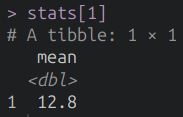
\includegraphics{img/mean.png}
    \end{center}

    \subsubsection{Odchylenie standardowe (standard deviation)}

    Odchylenie standardowe zostało obliczone przy pomocy funkcji \texttt{sd(value)}. Wzór:

    \Large
    \[
    s = \sqrt{\frac{1}{n - 1} \sum_{i=1}^{n}(x_i - \bar{x})^2}
    \]
    \normalsize

    \noindent gdzie:
    \begin{itemize}
    \item \( s \) -- odchylenie standardowe,
    \item \( x_i \) -- wartość obserwacji,
    \item \( \bar{x} \) -- średnia arytmetyczna,
    \item \( n \) -- liczba obserwacji.
    \end{itemize}

    \begin{center}
        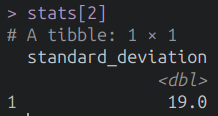
\includegraphics{img/sd.png}
    \end{center}

    \subsubsection{Współczynnik zmienności (coefficient of variation)}

    Został obliczony jako iloraz odchylenia standardowego i średniej:

    \Large
    \[
    CV = \frac{s}{\bar{x}}
    \]
    \normalsize

    \noindent gdzie:
    \begin{itemize}
    \item \( CV \) -- współczynnik zmienności,
    \item \( s \) -- odchylenie standardowe,
    \item \( \bar{x} \) -- średnia.
    \end{itemize}

    W R: \texttt{sd(value) / mean(value)}

    \begin{center}
        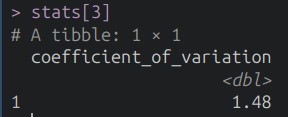
\includegraphics{img/cv.png}
    \end{center}

    \newpage

    \subsubsection{Kwantyle (kwartyle, mediana, min, max)}

    Obliczenia dokonane za pomocą funkcji \texttt{quantile(value)} oraz \texttt{min(value)}, \texttt{max(value)}. W R uwzględniłem:

    \begin{itemize}
        \item Q1: \texttt{quantile(value, 0.25)}
        \item Mediana (Q2): \texttt{quantile(value, 0.5)}
        \item Q3: \texttt{quantile(value, 0.75)}
        \item Minimum: \texttt{min(value)}
        \item Maksimum: \texttt{max(value)}
    \end{itemize}

    \begin{center}
        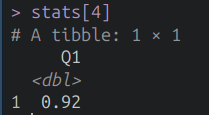
\includegraphics[scale=0.8]{img/q1.png} \\
        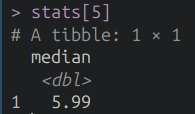
\includegraphics[scale=0.8]{img/q2.png} \\
        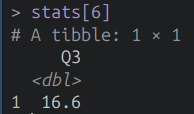
\includegraphics[scale=0.8]{img/q3.png} \\
        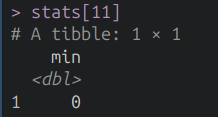
\includegraphics[scale=0.8]{img/min.png} \\
        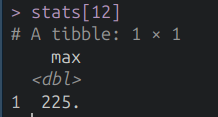
\includegraphics[scale=0.8]{img/max.png} \\
    \end{center}

    \begin{center}
        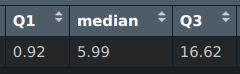
\includegraphics{img/quantiles.png}
    \end{center}

    \subsubsection{MAD (Median Absolute Deviation)}

    Odporna miara zmienności obliczona funkcją \texttt{mad(value)}. Wzór:

    \large
    \[
    MAD = \text{median}(|x_i - \text{median}(x)|)
    \]
    \normalsize

    \noindent gdzie:
    \begin{itemize}
    \item \( MAD \) -- medianowe odchylenie bezwzględne,
    \item \( x_i \) -- wartość obserwacji,
    \item \( \text{median}(x) \) -- mediana zbioru danych.
    \end{itemize}

    \begin{center}
        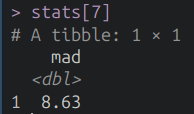
\includegraphics{img/mad.png}
    \end{center}

    \subsubsection{Odchylenie przeciętne (average deviation)}

    Średnia wartość bezwzględna odchyleń od średniej:

    \large
    \[
    \text{Average deviation} = \frac{1}{n} \sum_{i=1}^{n} |x_i - \bar{x}|
    \]
    \normalsize

    \noindent gdzie:
    \begin{itemize}
    \item \( x_i \) -- wartość obserwacji,
    \item \( \bar{x} \) -- średnia arytmetyczna,
    \item \( n \) -- liczba obserwacji.
    \end{itemize}

    W R: \texttt{mean(abs(value - mean(value)))}

    \begin{center}
        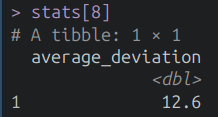
\includegraphics{img/avgdev.png}
    \end{center}

    \newpage

    \subsubsection{Dominanta (moda)}

    Wyznaczona za pomocą mojej własnej funkcji \texttt{get\_mode()}, która identyfikuje najczęściej występującą wartość w zbiorze:

    \begin{verbatim}
    get_mode <- function(v) {
    uniqv <- unique(v)
    uniqv[which.max(tabulate(match(v, uniqv)))]
    }
    \end{verbatim}

    \begin{center}
        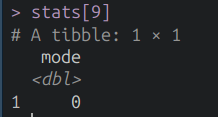
\includegraphics{img/mode.png}
    \end{center}

    \subsubsection{Wariancja}

    Obliczona funkcją \texttt{var(value)}. Wzór:

    \Large
    \[
    s^2 = \frac{1}{n - 1} \sum_{i=1}^{n}(x_i - \bar{x})^2
    \]
    \normalsize

    \noindent gdzie:
    \begin{itemize}
    \item \( s^2 \) -- wariancja,
    \item \( x_i \) -- wartość obserwacji,
    \item \( \bar{x} \) -- średnia,
    \item \( n \) -- liczba obserwacji.
    \end{itemize}

    \begin{center}
        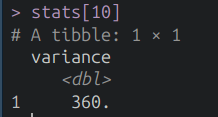
\includegraphics{img/variance.png}
    \end{center}

    \newpage

    \subsubsection{Rozstęp (range)}

    Obliczony jako różnica między maksimum a minimum:

    \large
    \[
    \text{Range} = \max(x) - \min(x)
    \]
    \normalsize

    \noindent gdzie:
    \begin{itemize}
    \item \( \max(x) \) -- największa wartość w zbiorze,
    \item \( \min(x) \) -- najmniejsza wartość w zbiorze.
    \end{itemize}

    W R: \texttt{max(value) - min(value)}

    \begin{center}
        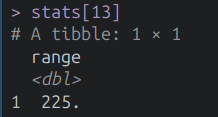
\includegraphics{img/range.png}
    \end{center}


    \subsubsection{Skośność (skewness)}

    Obliczona za pomocą funkcji \texttt{e1071::skewness(value)}. Wzór:

    \Large
    \[
    \text{Skewness} = \frac{\mu_3}{s^3}
    \]
    \normalsize

    \noindent gdzie:
    \begin{itemize}
    \item \( \mu_3 \) -- moment centralny rzędu 3,
    \item \( s \) -- odchylenie standardowe.
    \end{itemize}

    \begin{center}
        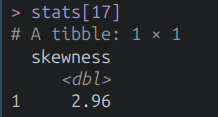
\includegraphics{img/skewness.png}
    \end{center}

    \newpage

    \subsubsection{Moment centralny rzędu 2, 3 i 4}

    Wszystkie trzy momenty zostały obliczone za pomocą mojej własnej funkcji \texttt{central\_moment(x, order)}:

    \begin{verbatim}
    central_moment <- function(x, order) {
    mean((x - mean(x))^order)
    }
    \end{verbatim}

    Ogólny wzór:

    \Large
    \[
    \mu_r = \frac{1}{n} \sum_{i=1}^{n} (x_i - \bar{x})^r
    \]
    \normalsize

    \noindent gdzie:
    \begin{itemize}
    \item \( \mu_r \) -- moment centralny rzędu \( r \),
    \item \( x_i \) -- wartość obserwacji,
    \item \( \bar{x} \) -- średnia,
    \item \( n \) -- liczba obserwacji,
    \item \( r \) -- rząd momentu (2, 3 lub 4).
    \end{itemize}

    \begin{itemize}
        \item \textbf{Rząd 2:} wariancja nieskorygowana,
        \item \textbf{Rząd 3:} miara asymetrii (surowa skośność),
        \item \textbf{Rząd 4:} miara kurtozy (surowa).
    \end{itemize}

    \begin{center}
        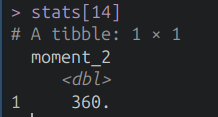
\includegraphics{img/moment2.png} \\
        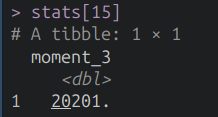
\includegraphics{img/moment3.png} \\
        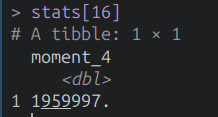
\includegraphics{img/moment4.png}
    \end{center}


    \subsection*{Podsumowanie}

    \begin{center}
      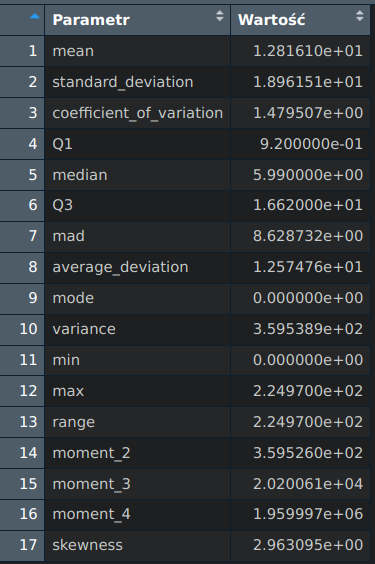
\includegraphics[scale=0.65]{img/parameters1.png}
    \end{center}

    \begin{center}
      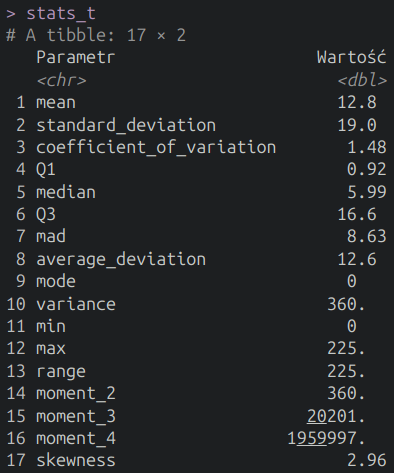
\includegraphics[scale=0.65]{img/parameters2.png}
    \end{center}

    \newpage

    \section{Wykresy - graficzna prezentacja danych}

    Dla lepszego zrozumienia struktury oraz zmienności współczynnika samobójstw na 100 tysięcy mieszkańców (\texttt{suicides/100k pop}), przygotowałem kilka wykresów ilustrujących rozkład oraz zależności między wybranymi cechami demograficznymi. Poniżej opisuję każdy z nich.

    \subsection{Histogram współczynnika samobójstw}

    \begin{figure}[H]
    \centering
    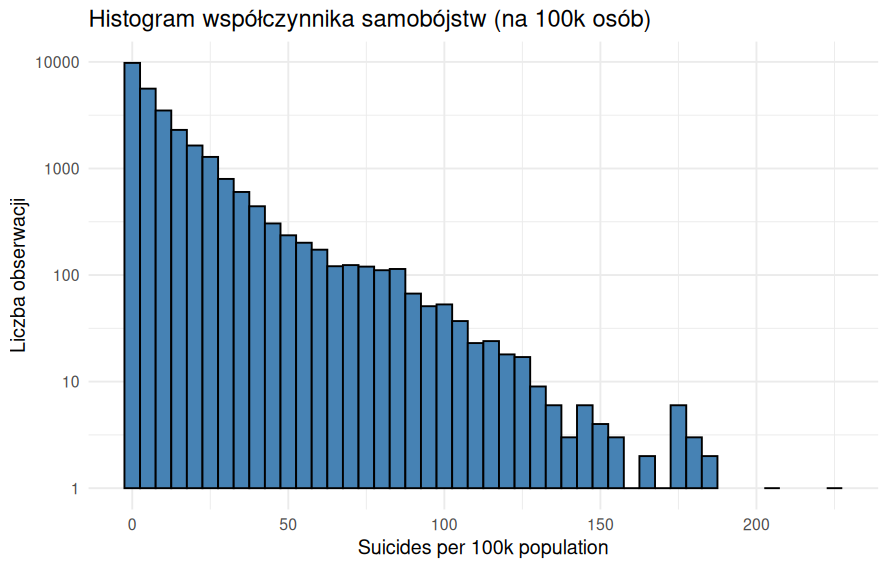
\includegraphics[width=0.7\textwidth]{img/histogram.png}
    \caption{Histogram współczynnika samobójstw (na 100k osób)}
    \end{figure}

    Histogram przedstawia rozkład wartości współczynnika samobójstw dla całego zbioru danych. Użyto podziału na przedziały o szerokości 5 jednostek. Oś X przedstawia liczbę samobójstw na 100 tysięcy osób, natomiast oś Y (w skali logarytmicznej) pokazuje liczbę obserwacji przypadających na dany przedział. Widać, że większość wartości mieści się w przedziale 0–30, co świadczy o koncentracji danych przy niskich wartościach współczynnika.

    \subsection{Wykres kołowy: średnia liczba samobójstw według płci}

    \begin{figure}[H]
    \centering
    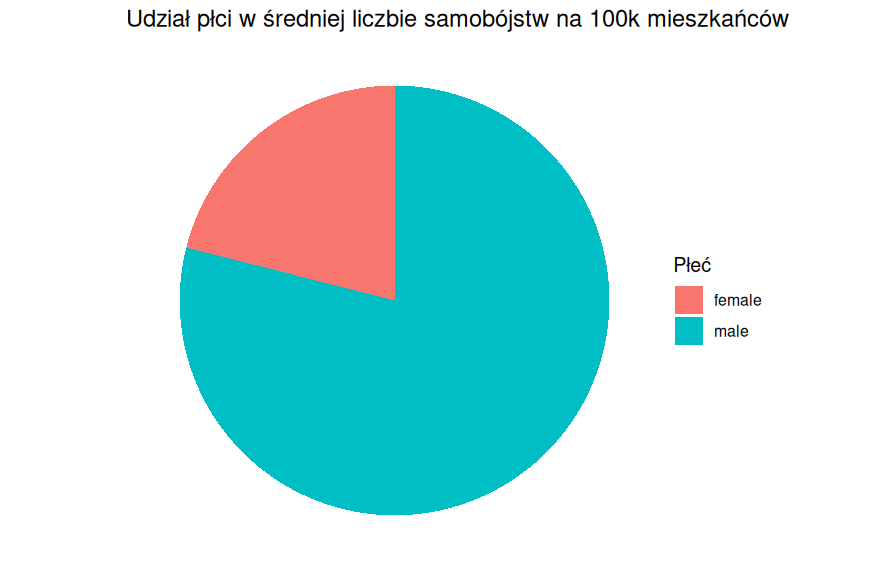
\includegraphics[width=0.5\textwidth]{img/pie_sex.png}
    \caption{Udział płci w średniej liczbie samobójstw na 100k mieszkańców}
    \end{figure}

    Wykres kołowy ilustruje udział mężczyzn i kobiet w średniej liczbie samobójstw na 100 tysięcy mieszkańców. Wartości zostały wyliczone jako średnia \texttt{value} w obrębie każdej płci, a następnie przeskalowane do udziałów procentowych. Wyniki jednoznacznie pokazują, że mężczyźni stanowią zdecydowaną większość przypadków, co jest zgodne z literaturą dotyczącą zjawiska samobójstw.

    \subsection{Wykres słupkowy: średnie samobójstwa według grup wiekowych}

    \begin{figure}[H]
    \centering
    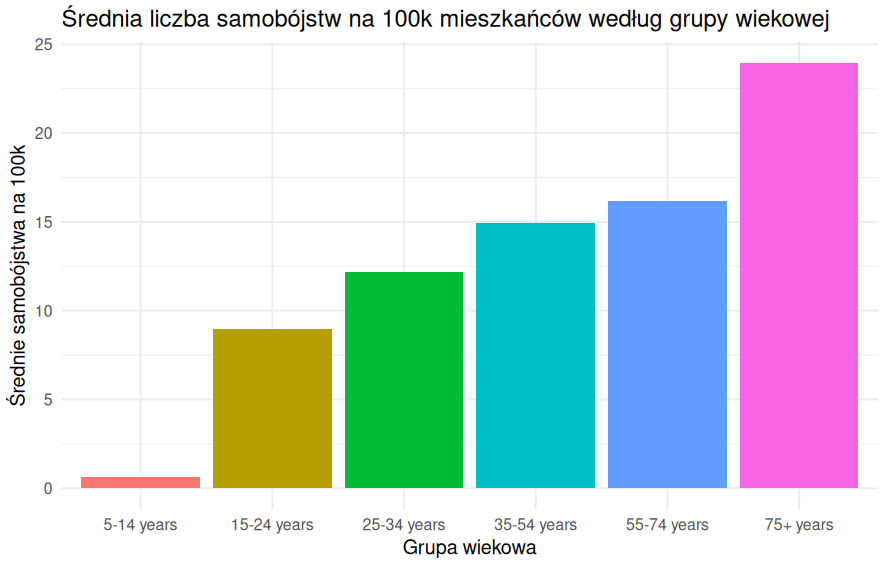
\includegraphics[width=0.8\textwidth]{img/bar_age.png}
    \caption{Średnia liczba samobójstw na 100k mieszkańców według grupy wiekowej}
    \end{figure}

    Wykres słupkowy pokazuje średnią wartość współczynnika samobójstw w podziale na sześć przedziałów wiekowych. Dane zostały odpowiednio uporządkowane rosnąco względem wieku. Zauważalna jest tendencja wzrostowa – starsze grupy wiekowe (zwłaszcza \texttt{75+ years}) charakteryzują się wyraźnie wyższym poziomem samobójstw w przeliczeniu na 100 tysięcy mieszkańców. Grupa \texttt{5-14 years} ma najniższe wartości, co jest zgodne z intuicją oraz danymi empirycznymi.

    \subsection{Mapa świata: średni współczynnik samobójstw według krajów}

    \begin{figure}[H]
    \centering
    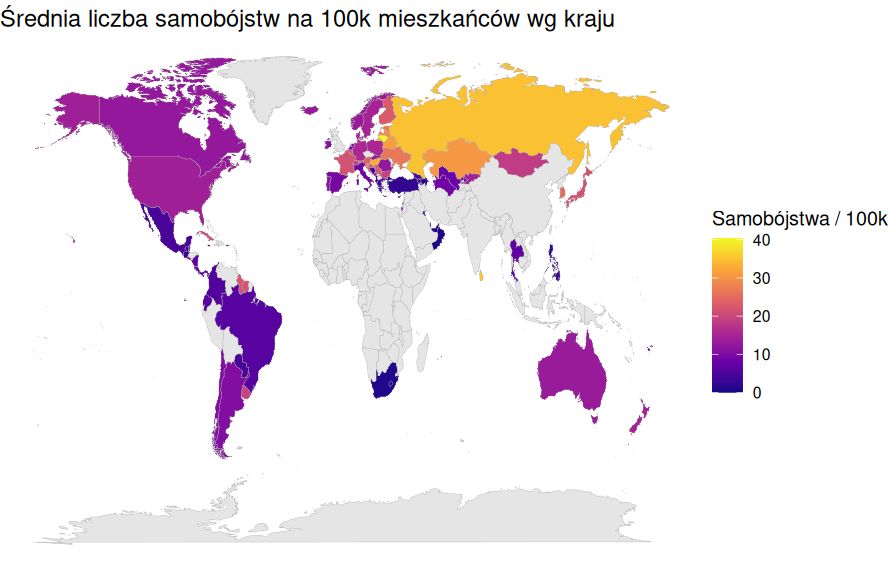
\includegraphics[width=\textwidth]{img/map.png}
    \caption{Średnia liczba samobójstw na 100k mieszkańców wg kraju}
    \end{figure}

    Mapa przedstawia przestrzenne zróżnicowanie współczynnika samobójstw między krajami. Dla każdego kraju obliczono średnią wartość \texttt{value}, a następnie odwzorowano ją kolorystycznie na mapie świata. Skala kolorów oparta jest na palecie \texttt{plasma} i została znormalizowana. Krajom bez danych przypisano jasnoszary kolor. Widać wyraźnie, że najwyższe wartości występują m.in. w Europie Wschodniej (np. Rosja, Litwa), a najniższe w krajach arabskich i w części Azji.

    \bigskip

    Powyższe wizualizacje umożliwiają wgląd w rozkład i dynamikę analizowanego zjawiska z różnych perspektyw: ogólnej (histogram), płciowej (wykres kołowy), wiekowej (słupkowy) oraz geograficznej (mapa). Graficzna reprezentacja danych potwierdza istotne zróżnicowanie współczynnika samobójstw w zależności od analizowanego wymiaru.


    \newpage

    \section{Hipotezy}

    W celu statystycznego zbadania właściwości danych oraz sprawdzenia istotnych różnic pomiędzy wybranymi grupami, postawiono dwie hipotezy badawcze. Zostały one zweryfikowane za pomocą odpowiednich testów statystycznych. Ponieważ wcześniejsza analiza wykazała, że dane nie mają rozkładu normalnego, zastosowano testy nieparametryczne, które nie wymagają spełnienia tego założenia.

    \subsection{Hipoteza 1: Czy rozkład \texttt{suicides/100k pop} jest normalny w podziale na płeć?}

    Celem tej analizy było sprawdzenie, czy dane dotyczące liczby samobójstw na 100 tysięcy mieszkańców dla mężczyzn i kobiet podlegają rozkładowi normalnemu.

    \begin{itemize}
        \item \( H_0 \): Rozkład \texttt{suicides/100k pop} dla danej płci jest normalny.
        \item \( H_1 \): Rozkład \texttt{suicides/100k pop} dla danej płci nie jest normalny.
    \end{itemize}

    Ponieważ zbiór danych zawiera ponad 27 tysięcy obserwacji, nie użyto testu Shapiro-Wilka, który ma ograniczenie do prób mniejszych niż 5000. Zamiast tego użyto testu Andersona-Darlinga, który jest bardziej odpowiedni dla dużych prób i pozwala ocenić zgodność rozkładu empirycznego z rozkładem normalnym.

    Wyniki testów zostały przedstawione poniżej. Dodatkowo, wskazano, czy wartość testu znajduje się w obszarze krytycznym (\( p < 0{,}05 \)):

    \begin{center}
        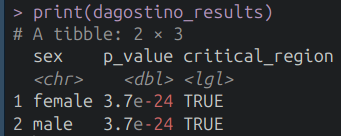
\includegraphics{img/hipoteza1.png}
    \end{center}

    \textbf{Interpretacja:}
    \begin{itemize}
        \item Jeżeli \( p < 0.05 \), odrzucamy hipotezę zerową — dane nie mają rozkładu normalnego, a wynik testu znajduje się w obszarze krytycznym.
        \item Jeżeli \( p \geq 0.05 \), brak podstaw do odrzucenia hipotezy — dane mogą pochodzić z rozkładu normalnego.
    \end{itemize}

    \textbf{Wniosek:} Dla obu płci uzyskano p-wartości mniejsze niż 0.05, co oznacza, że wyniki znajdują się w obszarze krytycznym. Odrzucamy hipotezę zerową i uznajemy, że rozkład danych nie jest normalny. Z tego względu w dalszej analizie zastosowano testy nieparametryczne.

    \subsubsection*{Test Andersona-Darlinga (Anderson-Darling normality test)}

    Test ten służy do sprawdzenia normalności danych, porównując rozkład empiryczny z rozkładem normalnym. Jest bardziej czuły niż test Shapiro-Wilka w przypadku dużych prób.

    \begin{itemize}
        \item Hipoteza zerowa (\(H_0\)): Dane pochodzą z rozkładu normalnego.
        \item Hipoteza alternatywna (\(H_1\)): Dane nie pochodzą z rozkładu normalnego.
    \end{itemize}

    Ze względu na charakter nieparametryczny, statystyka testu nie ma rozkładu łatwego do graficznej interpretacji. Dlatego przyjęto prostą zasadę: \textbf{jeśli p-value < 0.05, uznajemy wynik za istotny statystycznie (obszar krytyczny)}.

    \newpage

    \subsection{Hipoteza 2: Czy występuje istotna różnica w liczbie samobójstw między grupami wiekowymi \texttt{15-24 years} a \texttt{75+ years}?}

    Celem tego testu było sprawdzenie, czy poziom współczynnika samobójstw różni się istotnie między najmłodszą i najstarszą grupą wiekową.

    \begin{itemize}
        \item \( H_0 \): Rozkłady \texttt{suicides/100k pop} w grupach „15–24” i „75+” są takie same.
        \item \( H_1 \): Rozkłady różnią się istotnie.
    \end{itemize}

    Z uwagi na brak normalności rozkładu, zastosowano test U Manna-Whitneya (Wilcoxona), który porównuje mediany dwóch niezależnych prób. Test ten nie wymaga założenia normalności ani równości wariancji.

    \textbf{Interpretacja:}
    \begin{itemize}
        \item Jeżeli \( p < 0.05 \), odrzucamy hipotezę zerową — różnica jest istotna, a wynik testu leży w obszarze krytycznym.
        \item Jeżeli \( p \geq 0.05 \), brak podstaw do stwierdzenia różnicy.
    \end{itemize}

    \textbf{Wyniki:}

    \begin{center}
        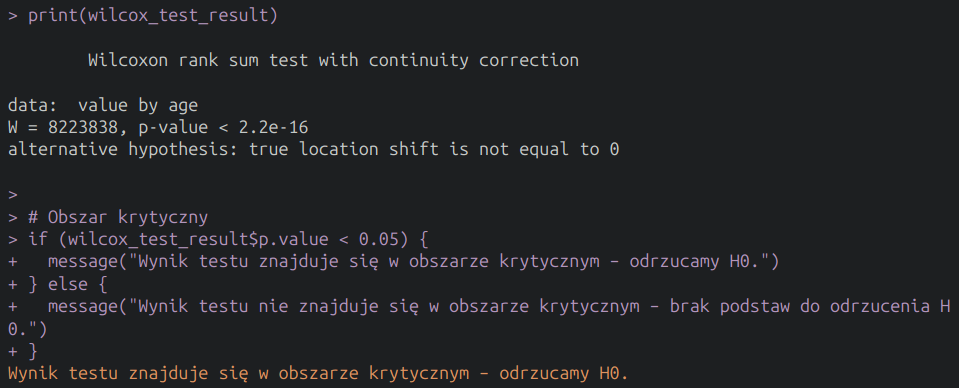
\includegraphics[scale=0.52]{img/hipoteza2.png}
    \end{center}

    \begin{center}
        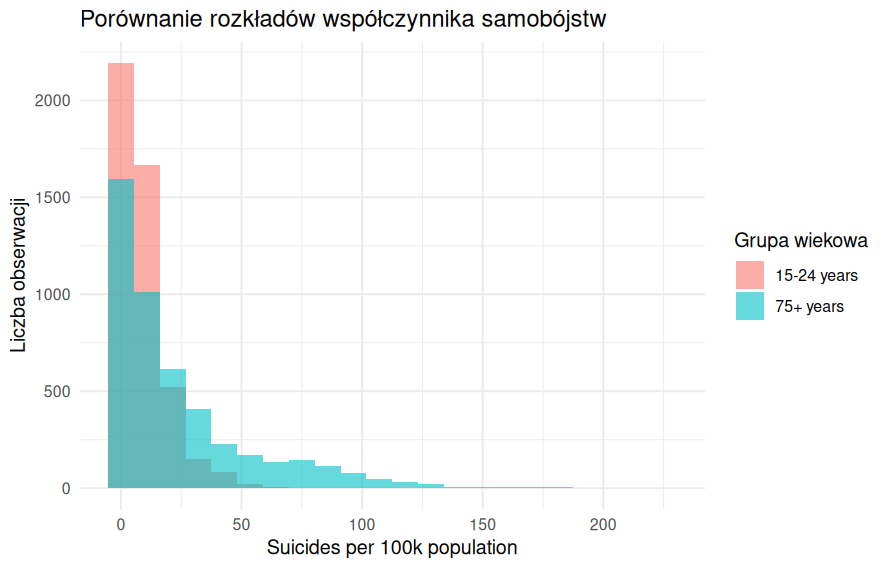
\includegraphics[scale=0.75]{img/histogram_hipoteza2.png}
    \end{center}

    Histogram powyżej przedstawia rozkład współczynnika samobójstw w obu porównywanych grupach wiekowych. Pomaga on wizualnie dostrzec różnice, które potwierdzono statystycznie.

    \textbf{Wniosek:} p-wartość jest znacznie mniejsza niż 0.05, co oznacza, że wynik testu znajduje się w obszarze krytycznym. Odrzucamy hipotezę zerową i stwierdzamy istotną statystycznie różnicę w poziomie współczynnika samobójstw pomiędzy młodą a starszą grupą wiekową. Starsze osoby (\texttt{75+ years}) są znacznie bardziej zagrożone.

    \subsubsection*{Test Manna-Whitneya (Wilcoxona)}

    Jest to test nieparametryczny służący do porównywania dwóch niezależnych prób. Stanowi alternatywę dla testu t-Studenta, gdy nie można przyjąć normalności rozkładów.

    \begin{itemize}
        \item Hipoteza zerowa (\(H_0\)): Obie grupy pochodzą z tej samej populacji (rozkłady są identyczne).
        \item Hipoteza alternatywna (\(H_1\)): Rozkłady różnią się istotnie.
    \end{itemize}

    Również w tym przypadku nie wizualizuje się rozkładu statystyki testowej bezpośrednio, lecz opiera się interpretację na p-wartości i jej relacji względem poziomu istotności.

    W R test wykonano za pomocą funkcji \texttt{wilcox.test()}, a obszar krytyczny wyznaczono na poziomie \( \alpha = 0.05 \).

    \bigskip

    \textbf{Podsumowanie:}
    Oba testy zostały świadomie dobrane jako nieparametryczne ze względu na charakter danych. Analizy wykazały brak normalności rozkładów oraz istotną różnicę między wybranymi grupami. Dla obu hipotez decyzja o odrzuceniu \( H_0 \) była oparta na p-wartości znajdującej się w obszarze krytycznym.

    \newpage

    \section{Wnioski}

    Celem niniejszej analizy było statystyczne opisanie i zinterpretowanie zjawiska samobójstw w oparciu o dane międzynarodowe z lat 1985–2016. W toku pracy wykonano szereg działań analitycznych — od eksploracji danych, przez wyznaczenie podstawowych parametrów opisowych, aż po testowanie hipotez statystycznych.

    \subsection*{Najważniejsze obserwacje}

    \begin{itemize}
        \item Dane charakteryzują się dużym zróżnicowaniem względem płci, wieku oraz krajów.
        \item Zmienna \texttt{suicides/100k pop} nie ma rozkładu normalnego — co wykazano za pomocą testu Andersona-Darlinga — co uzasadniło zastosowanie testów nieparametrycznych w dalszych analizach.
        \item Mężczyźni stanowią zdecydowaną większość przypadków samobójstw, co jest zgodne z doniesieniami epidemiologicznymi.
        \item Wiek ma istotny wpływ na poziom współczynnika samobójstw. Najwyższe wartości występują w grupie \texttt{75+ years}, co potwierdzono statystycznie testem Manna-Whitneya.
        \item Graficzna analiza danych (histogramy, wykresy słupkowe, mapa) umożliwiła wgląd w strukturę zjawiska oraz potwierdziła wnioski płynące z analiz liczbowych.
    \end{itemize}

    \subsection*{Wnioski końcowe}

    Analiza potwierdziła zróżnicowanie ryzyka samobójstw w zależności od płci i wieku. Zidentyfikowano grupy szczególnie narażone (mężczyźni, osoby starsze), co może stanowić ważny punkt odniesienia dla dalszych badań lub działań profilaktycznych.

    Zastosowane metody statystyczne pozwoliły nie tylko opisać dane, ale również zweryfikować hipotezy na podstawie wiarygodnych i odpornych na założenia testów. Całość analizy została przeprowadzona w sposób przejrzysty, z naciskiem na transparentność obliczeń i interpretacji.

    \bigskip

    Zestawienie obliczonych parametrów oraz wykonanych testów, uzupełnione o odpowiednie wizualizacje, stanowi pełny i spójny obraz statystyczny badanego zjawiska.

    \newpage

    \section{Listing komend}

    \subsection{Użyte biblioteki}

    W projekcie wykorzystano następujące biblioteki języka R:

    \begin{itemize}
        \item \texttt{tidyverse} -- zestaw bibliotek do manipulacji danymi (\texttt{dplyr}, \texttt{ggplot2}, \texttt{readr}, itp.),
        \item \texttt{patchwork} -- umożliwia łączenie wielu wykresów w jeden układ,
        \item \texttt{rio} -- uproszczony import i eksport danych (m.in. CSV),
        \item \texttt{ggthemes} -- dodatkowe motywy do wykresów \texttt{ggplot2},
        \item \texttt{kaggler} -- autorska biblioteka do integracji z API Kaggle,
        \item \texttt{dotenv} -- ładowanie zmiennych środowiskowych z pliku \texttt{.env},
        \item \texttt{reticulate} -- interfejs do korzystania z języka Python wewnątrz R,
        \item \texttt{e1071} -- statystyka i uczenie maszynowe; zawiera funkcję \texttt{skewness()},
        \item \texttt{maps} -- dane geograficzne potrzebne do tworzenia map,
        \item \texttt{nortest} -- testy normalności, w tym test Andersona-Darlinga.
    \end{itemize}

    \subsection{Użyte funkcje}

    Poniżej wyszczególniono wszystkie funkcje użyte w kodzie, z przypisaniem do odpowiednich bibliotek:

    \begin{itemize}
        \item \texttt{system()} -- (bazowy R) wykonanie komendy systemowej, np. \texttt{pwd}, \texttt{mkdir}, \texttt{mv}.
        \item \texttt{paste()} -- (bazowy R) łączenie tekstów w jeden ciąg znaków.
        \item \texttt{setwd()} -- (bazowy R) ustawienie katalogu roboczego.
        \item \texttt{load\_dot\_env()} -- z biblioteki \texttt{dotenv}; ładowanie zmiennych środowiskowych.
        \item \texttt{kgl\_auth\_file\_setup()} -- z biblioteki \texttt{kaggler}; konfiguracja uwierzytelnienia.
        \item \texttt{install\_python()} -- z \texttt{reticulate}; instalacja wersji Pythona.
        \item \texttt{virtualenv\_create()} -- z \texttt{reticulate}; tworzenie środowiska wirtualnego.
        \item \texttt{virtualenv\_install()} -- z \texttt{reticulate}; instalacja pakietów w środowisku.
        \item \texttt{use\_virtualenv()} -- z \texttt{reticulate}; aktywacja środowiska.
        \item \texttt{import()} -- z \texttt{reticulate}; import modułu z Pythona.
        \item \texttt{read\_csv()} -- z \texttt{readr}; wczytywanie pliku CSV.
        \item \texttt{rename\_with()} -- z \texttt{dplyr}; zmiana nazw kolumn.
        \item \texttt{str\_trim()} -- z \texttt{stringr}; usuwanie białych znaków.
        \item \texttt{str\_subset()} -- z \texttt{stringr}; wybór elementów wektora pasujących do wzorca.
        \item \texttt{str\_replace\_all()} -- z \texttt{stringr}; zamiana znaków w ciągu znaków.
        \item \texttt{as.numeric()} -- (bazowy R) konwersja do typu numerycznego.
        \item \texttt{drop\_na()} -- z \texttt{tidyr}; usunięcie wierszy zawierających wartości \texttt{NA}.
        \item \texttt{unique()} -- (bazowy R) znalezienie unikalnych wartości.
        \item \texttt{match()} -- (bazowy R) dopasowanie wartości.
        \item \texttt{tabulate()} -- (bazowy R) zliczanie liczby wystąpień.
        \item \texttt{which.max()} -- (bazowy R) indeks największej wartości.
        \item \texttt{mean()} -- (bazowy R) obliczanie średniej.
        \item \texttt{sd()} -- (bazowy R) obliczanie odchylenia standardowego.
        \item \texttt{quantile()} -- (bazowy R) obliczanie kwantyli.
        \item \texttt{mad()} -- (bazowy R) obliczanie medianowego odchylenia bezwzględnego.
        \item \texttt{abs()} -- (bazowy R) wartość bezwzględna.
        \item \texttt{var()} -- (bazowy R) wariancja.
        \item \texttt{min()} / \texttt{max()} -- (bazowy R) wartości skrajne.
        \item \texttt{summarise()} -- z \texttt{dplyr}; podsumowanie danych.
        \item \texttt{group\_by()} -- z \texttt{dplyr}; grupowanie danych.
        \item \texttt{ungroup()} -- z \texttt{dplyr}; usuwanie grupowania.
        \item \texttt{mutate()} -- z \texttt{dplyr}; tworzenie/zmiana kolumn.
        \item \texttt{rename()} -- z \texttt{dplyr}; zmiana nazw kolumn.
        \item \texttt{filter()} -- z \texttt{dplyr}; filtrowanie wierszy.
        \item \texttt{select()} -- z \texttt{dplyr}; wybór kolumn.
        \item \texttt{print()} -- (bazowy R) wyświetlanie wyników.
        \item \texttt{message()} -- (bazowy R) wypisanie komunikatu tekstowego.
        \item \texttt{ggplot()} -- z \texttt{ggplot2}; tworzenie wykresów.
        \item \texttt{aes()} -- z \texttt{ggplot2}; definicja estetyki wykresu.
        \item \texttt{geom\_histogram()} -- z \texttt{ggplot2}; wykres histogramu.
        \item \texttt{geom\_col()} -- z \texttt{ggplot2}; słupki (barplot, pie).
        \item \texttt{coord\_polar()} -- z \texttt{ggplot2}; przekształcenie do wykresu kołowego.
        \item \texttt{theme\_minimal()} / \texttt{theme\_void()} -- z \texttt{ggthemes}; styl wykresu.
        \item \texttt{labs()} -- z \texttt{ggplot2}; opisy osi i tytułów.
        \item \texttt{theme()} -- z \texttt{ggplot2}; ustawienia wyglądu wykresu.
        \item \texttt{scale\_y\_log10()} -- z \texttt{ggplot2}; logarytmiczna skala osi Y.
        \item \texttt{map\_data()} -- z \texttt{maps}; dane do mapy świata.
        \item \texttt{left\_join()} -- z \texttt{dplyr}; łączenie danych.
        \item \texttt{geom\_polygon()} -- z \texttt{ggplot2}; rysowanie wielokątów mapy.
        \item \texttt{scale\_fill\_viridis\_c()} -- z \texttt{ggplot2} (lub viridis); kolorystyka ciągła.
        \item \texttt{ad.test()} -- z \texttt{nortest}; test Andersona-Darlinga.
        \item \texttt{wilcox.test()} -- (bazowy R) test Manna-Whitneya (Wilcoxona).
    \end{itemize}

    \subsubsection*{Funkcje własne}

    W kodzie zdefiniowano również dwie funkcje autorskie:

    \begin{itemize}
        \item \texttt{get\_mode(v)} -- zwraca najczęściej występującą wartość w zbiorze.
        \item \texttt{central\_moment(x, order)} -- oblicza moment centralny dowolnego rzędu.
    \end{itemize}

    \newpage


\end{document}
